\documentclass{beamer}

\usetheme{madrid}
\date{\today}
\institute{UNNC}
\title{My Presentation}
\author{HAMOOD}
\begin{document}
%*****************************
\begin{frame} % Frame 1
\maketitle
\end{frame}
%*****************************
\begin{frame} % Frame 2
\frametitle{Outlines}
\tableofcontents
\end{frame}
%*****************************


\section{Introduction}
\begin{frame} % Frame 3
\frametitle{First order derivative}
\begin{block}{Stationary Point}
$x_0$ is a stationary point of $f(x)$ if $f'(x_0) = 0$
\end{block}



\end{frame}
%*****************************
\begin{frame} % Frame 4
\frametitle{First order derivative}

If $x_0$ is a stationary point of $y = f (x)$, then $f (x)$ may achieve its maximum/minimum value at $x = x0$.\\\pause
\begin{block}{Second Derivative Test}
\begin{itemize}
\item
If $f''(x0) < 0$, then f has maximum value at $x = x_0$.
\item
If $f''(x0) > 0$, then f has minimum value at $x = x_0$.
\end{itemize}
\end{block}


\end{frame}
%*****************************
\section{Example}
\begin{frame} % Frame 5
\frametitle{Question}
Find the (local) \textbf{maximum/minimum} values of function
\begin{equation*}
f (x) = 3x^4 - 20x^3 + 36x^2 - 15
\end{equation*}
\underline{Solution:}
\begin{eqnarray}
f'(x) &=& 12x3 - 60x2 + 72x (1)\\
f''(x) &=& 36x2 - 120x + 72 
\end{eqnarray}

$f'(x)$ = 0 $\Rightarrow$ x = 0, 2, 3 are stationary points of $f (x)$.
\end{frame}
%*****************************
\begin{frame} % Frame 6
\frametitle{Cont’d}
Below is a table for summarizing the test result:
\begin{table}\center\begin{tabular}{|l|c|l|}\hline
$(x_0, f (x_0))$ &$ f''(x)|_{x=x_0}$&classification\\\hline
(0, -15)&> 0&point of minimum\\\hline
(2, 17) &< 0& point of maximum\\\hline
(3, 12) &> 0& point of minimum\\\hline
\end{tabular}
\caption{Second Derivative Test}
\end{table}
\end{frame}
%*****************************
\begin{frame} % Frame 7
\frametitle{Function plot}
Below is a plot of y = f (x) in \textbf{GeoGebra}:
\begin{figure}
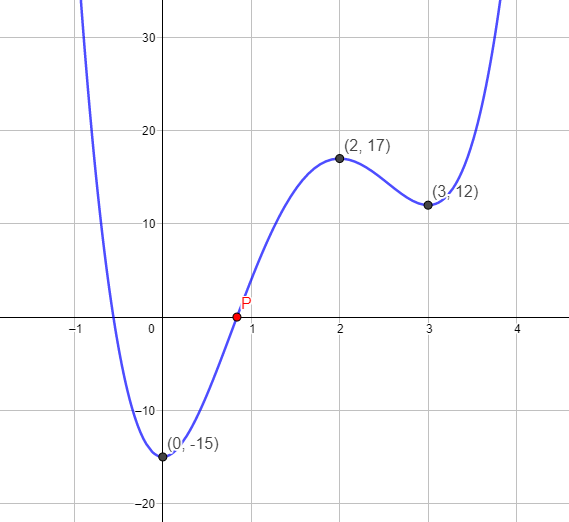
\includegraphics[scale=0.4]{polynomial}
\caption{$f (x) = 3x^4 - 20x^3 + 36x^2 - 15$}
\end{figure}


\end{frame}
%*****************************
\section{Application}
\begin{frame} % Frame 8
\frametitle{N-R method}
Use \underline{Newton-Raphson Method} to find one apporximate root at P (correct to 5 d.p.), with $x_0 = 1$.
\begin{columns}
\column{0.6\textwidth}
\begin{eqnarray}
x_{n+1}&=&x_n-\frac{f(x_n)}{f'(x_n)}\\
&=&\cdots\nonumber\\
&=&\frac{9x^4_n - 40x^3_n + 36x^2_n + 15}{12x^3_n - 60x^2_n + 72x_n}
\end{eqnarray}
\column{0.4\textwidth}
\begin{tabular}{|c|c|}
n&$x_n$\\
0&1.0000\\
1 &0.8333\\
2 &0.8384\\
3 &0.8384\\
\end{tabular}
\end{columns}
\vfill
$\therefore$ the desired root $x^* = 0.8384.$

\end{frame}
%*****************************
\begin{frame}[fragile] % Frame 9
\frametitle{Remark}
The iteration formula in \hyperlink{frame8}{\beamerbutton{previous frame}} is typeset by the following command lines:
\begin{verbatim}
\begin{eqnarray}
x_{n+1}&=& x_n-\frac{f(x_n)}{f’(x_n)}\\[1ex]
&=& \cdots \nonumber\\[1ex]
&=& \frac{9x_n^4-40x_n^3+36x_n^2+15}{12x_n^3-60x_n^2+72x_n}
\end{eqnarray}
\end{verbatim}
\end{frame}
%*****************************
\begin{frame} % Frame 10
\frametitle{Q\&A}
\textbf{Thank you!}

Any questions?
\end{frame}
%*****************************
\end{document}